\chapter{Sleep Database and Sleep Stage Classification Algorithm}
\label{chapter:data_and_algorithm}

This chapter describes the Cyclic Alternating Pattern (CAP) Sleep Database used and the algorithm implemented. The algorithm uses FFT, PCA and $k$-nearest-neighbor to estimate the sleep stage from a recorded EEG signal.

We use the CAP Sleep Database~\cite{Terzano2001}\cite{Goldberger2000} which provides 16 recordings of patients without pathology. Two of these recordings have corrupted files and one did not record the data points used for this analysis and thus could not be analyzed. Table~\ref{tab:meta_data_of_recordings} shows some meta data of the recordings.

\begin{table}[h]
	\centering
	\begin{tabular}{c|c|c|c|c|c}
		File Name & Age & Gender & Length of Recording & Channel Name & Sampling Frequency \\
		\hline
		n1  & 37 & F & 577 minutes & C4-A1  & 512 Hz \\
		n2  & 34 & M & 735 minutes & C4-A1  & 512 Hz \\
		n3  & 35 & F & 551 minutes & C4-A1  & 512 Hz \\
		n4  & 25 & F & 596 minutes & C4-A1  & 200 Hz \\
		n5  & 35 & F & 524 minutes & C4-A1  & 512 Hz \\
		n6  & 31 & M & 527 minutes & C3-A2  & 128 Hz \\
		n7  & 31 & M & 492 minutes & C3-A2  & 128 Hz \\
		n8  & 42 & F & 501 minutes & C3-A2  & 200 Hz \\
		n9  & 31 & M & 532 minutes & C3-A2  & 128 Hz \\
		n10 & 23 & M & 490 minutes & C4-A1  & 512 Hz \\
		n11 & 28 & F & 527 minutes & C4-A1  & 512 Hz \\
		n12 & 29 & M & 495 minutes & C3-A2  & 100 Hz \\
		n16 & 41 & F & 513 minutes & C4-A1  & 100 Hz \\
	\end{tabular}
	\caption{Meta data of the 13 recordings from the CAP Sleep Database.}
	\label{tab:meta_data_of_recordings}
\end{table}

The given dataset describes multiple channels of EEG data recorded during sleep. We are interested in the channels recording activity in the central area, as these are the two channels most of the recordings share. Figure~\ref{fig:head_placement} shows where the sensors were placed. Other channels recorded activity in the frontal area, but are not used as mixing different channels poses problems in comparability between recordings.

\begin{figure}[h]
	\centering
	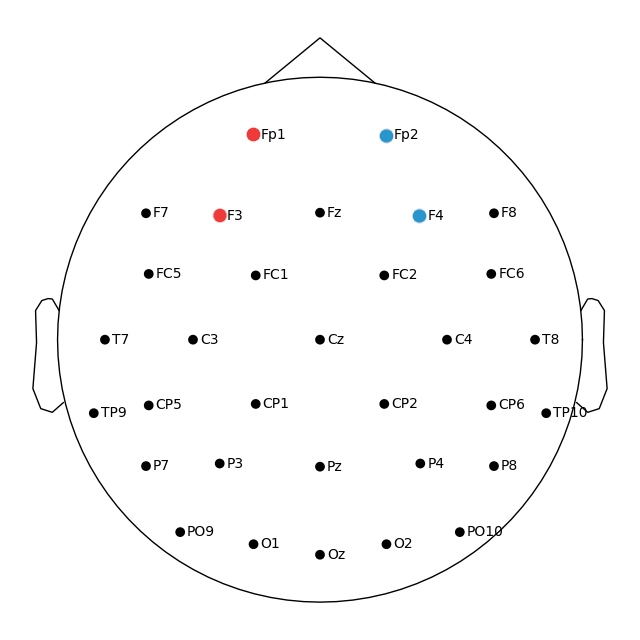
\includegraphics[width=0.6\linewidth]{figs/head_placement}
	\caption{Scheme of sensor placement in recordings of EEG data.}
	\label{fig:head_placement}
\end{figure}

\newpage
The data was recorded with different sampling frequencies. To reduce data size and standardize all channels we resample to 200 Hz.

Frequencies lower than 0.5 Hz and higher than 30 Hz often stem from other sources, such as the measurement equipment, breathing of the patients or measuring inaccuracies. To remove these noises from the data we want to remove these very low and very high frequencies from the recordings. We do this by applying a low pass filter of 30 Hz and a high pass filter of 0.5 Hz before using the data.

We now describe the general structure of the algorithm from reading the data files to the clustering.

The EEG data is stored in European data format (EDF) files. They provide a standard for exchanging and storing medical time-series data.

First we split the recorded data into 30 second sections, as is common in sleep stage classification. For each of these sections we get the data as a function of amplitude over time. An example segment is shown in the upper figure of~\ref{fig:example_30s_segment}. We apply a Fourier transformation as described in section~\ref{sec:fourier_transformation} and get a function of amplitude over frequency. This gives a frequency based representation of the data. As the sleep stages are characterized by different frequencies and amplitudes, as described in chapter~\ref{chapter:introduction}, this will help us to distinguish them. The output of such an FFT can be seen in the lower figure of~\ref{fig:example_30s_segment}. The pseudo code for this processing is presented in algorithm~\ref{alg:process_eeg_data}.
\newpage

\begin{figure}[h]
	\centering	
	\begin{subfigure}[b]{\textwidth}
		\begin{tikzpicture}
			\begin{axis}[xlabel=Time, x unit=\si\second, ylabel=Amplitude, width=\textwidth, height=0.3\textwidth]
				\addplot+ [no marks, color=black] table[col sep=comma] {figs/example_30s_segment1.csv};
			\end{axis}
		\end{tikzpicture}
	\end{subfigure}
	\vskip\baselineskip
	\begin{subfigure}[b]{\textwidth}
		\begin{tikzpicture}
			\begin{axis}[xlabel=Frequency, x unit=\si\hertz, ylabel=Amplitude, width=\textwidth, height=0.3\textwidth]
				\addplot+ [no marks, color=black] table[col sep=comma] {figs/example_30s_segment2.csv};
			\end{axis}
		\end{tikzpicture}
	\end{subfigure}
	
	\caption{A 30 second segment of the data. The top shows the recorded signal of the EEG. The bottom shows the output of the Fourier transformation.}
	\label{fig:example_30s_segment}
\end{figure}

\begin{algorithm}[h!]
	\caption{EEG data processing}\label{alg:process_eeg_data}
	\begin{algorithmic}
		\For{each patient}
		\State Read EEG data from file
		\State Apply a 30 Hz low pass and a 0.5 Hz high pass filter
		\State Resample with frequency 200 Hz
		\State Get one of the channels C4-A1 or C3-A2 (in this order)
		\State Section out the part of data where the patient is asleep
		\For{each 30 second segment of the data}
		\State Do a Fourier transformation (FFT)
		\EndFor
		\State Save all the outputs from the FFT to the patients file
		\EndFor
	\end{algorithmic}
\end{algorithm}

We now have high dimensional data points, as each 30 second segment is represented by the amplitudes for each of the distinct frequencies output by the FFT. Before we can start finding the clusters in the data we want to find a lower dimensional representation. This is were PCA can be used.

\newpage

We now show pseudo code of the part of our algorithm, which takes labeled data to derive information, to be used later. This information enables the other part of the algorithm to label previously unlabeled data. This is the training phase and is only needed to be run once.

\begin{algorithm}[h!]
	\caption{Apply PCA to the EEG data}\label{alg:pca_of_eeg_data}
	\begin{algorithmic}
		\For{each patient}
		\State Read FFT output from patients file
		\State Read sleep stages from another file
		\EndFor
		\State Concatenate FFT data of all patients
		\State Concatenate sleep stages of all patients
		\State Do PCA on the combined FFT data
		\State Transform data according to the principal components from the PCA
		\State Visualize the data in the first three axis, with the color corresponding to the sleep stage
	\end{algorithmic}
\end{algorithm}

From the output of algorithm~\ref{alg:pca_of_eeg_data} we get principal components, which reveal the frequencies were the most variance is shown. Under our assumptions this variation is caused by the different sleep stages of the different segments in the recording. We show a visual representation of the data in the first three principal components in figure~\ref{fig:pca_output_3d}.

\vspace{0.5cm}

\begin{figure}[h]
	\centering	
	\begin{tikzpicture}
		\begin{axis}[xlabel=PC 1, ylabel=PC 2, zlabel=PC 3, width=0.8\textwidth, height=0.3\textwidth, view/az=-45, view/el=45, legend entries={awake, REM, S3, S2, S1}, legend pos=outer north east, z post scale=3.5]
			\addplot3+ [only marks, mark=x, red] table[col sep=comma] {figs/pca_output_3d_stage_awake.csv};
			\addplot3+ [only marks, mark=x, black] table[col sep=comma] {figs/pca_output_3d_stage_REM.csv};			
			\addplot3+ [only marks, mark=x, blue] table[col sep=comma] {figs/pca_output_3d_stage_S3.csv};		
			\addplot3+ [only marks, mark=x, green] table[col sep=comma] {figs/pca_output_3d_stage_S2.csv};
			\addplot3+ [only marks, mark=x, yellow] table[col sep=comma] {figs/pca_output_3d_stage_S1.csv};
		\end{axis}
	\end{tikzpicture}	
	\caption{Three dimensional representation of the data. Each 30 second segment is represented by a cross in the color corresponding to the sleep stage this segment is assigned to.}
	\label{fig:pca_output_3d}
\end{figure}

\newpage
If we have a new recording and want to know the sleep stages we have to follow similar steps. First, the recording has to be split into 30 second segments. These have to be transformed by a FFT. The output can be converted to the PCA basis by multiplying with the matrix of principal components. Lastly, we can get an estimate of the sleep stage by using the $k$-nearest-neighbor algorithm. The pseudo code is shown in algorithm~\ref{alg:gues_sleep_stage}.

\begin{algorithm}[h]
	\caption{Get estimate for sleep stage}\label{alg:gues_sleep_stage}
	\begin{algorithmic}
		\Require{EEG recording of sleep}
		\For{each 30s segment}
			\State Apply FFT to the segment
			\State Multiply FFT output by principal component matrix
			\State Reduce dimensions
			\State Apply $k$-nearest-neighbor
			\State Save the result of $k$-nearest-neighbor
		\EndFor
		\State \Return results of $k$-nearest-neighbor
	\end{algorithmic}
\end{algorithm}

For every EEG recording which we want to label we need to run Algorithm~\ref{alg:gues_sleep_stage}.
